% This must be in the first 5 lines to tell arXiv to use pdfLaTeX, which is strongly recommended.
\pdfoutput=1
% In particular, the hyperref package requires pdfLaTeX in order to break URLs across lines.

\documentclass[11pt]{article}

% Remove the "review" option to generate the final version.
\usepackage[]{acl}

% Standard package includes
\usepackage{times}
\usepackage{latexsym}

% For proper rendering and hyphenation of words containing Latin characters (including in bib files)
\usepackage[T1]{fontenc}
% For Vietnamese characters
% \usepackage[T5]{fontenc}
% See https://www.latex-project.org/help/documentation/encguide.pdf for other character sets

% This assumes your files are encoded as UTF8
\usepackage[utf8]{inputenc}

% This is not strictly necessary, and may be commented out,
% but it will improve the layout of the manuscript,
% and will typically save some space.
\usepackage{microtype}
\usepackage{graphicx}
\usepackage{xcolor}

% If the title and author information does not fit in the area allocated, uncomment the following
%
%\setlength\titlebox{<dim>}
%
% and set <dim> to something 5cm or larger.

\title{Investigating teaching rule based inference to LLMs}

\author{Julian Fesel \\
\texttt{julian.fesel@icloud.com}
}

\begin{document}
    \maketitle
    \begin{abstract}
        Brief statement providing context for your ideas, and then a high-level summary of what you did and its significance. This is a required section.
    \end{abstract}


    \section{Introduction}
    %This template uses the ACL 2022 style files.
    %The numbered section headings are merely suggestions. The two un-numbered sections at the end are required, as is a references section.
    %The maximum length of the paper is 8 pages, excluding the two required un-numbered sections, references, and appendices. There is no length limit for these additional sections. Appendices cannot report on core findings of the paper.
    %If you have additional questions about requirements for style, formatting, length, etc., please refer to the ACL guidelines: \url{https://acl-org.github.io/ACLPUB/formatting.html}. Unless otherwise specified, we will adopt their requirements.

    The motivation for this project comes from my current occupation in the railway sector.
    There, routing conflicts between different scheduled trains must be solved by special operatives.
    Most of these decisions follow guidelines that define which trains must be prioritized under which circumstances.

    These guidelines can be quite extensive and intricate and the decisions must be made quickly.
    It is therefore of interest, to try to use LLMs to support the operatives in this task, by providing decision
    recommendations based on the guidelines and a description of the current situation.

    Since the data that would be necessary to work on this topic is currently not available, this project aims to
    investigate a topic that is relevant to this future effort.
    There are three main topics that this project addresses:
    \begin{enumerate}
        \item What is the most efficient way to transform a small training dataset into performance of a model?
        \item What is the best way to teach a model to follow given guidelines?
        \item How do chain-of-thought style prompting and fine-tuning relate to each other?
    \end{enumerate}

    The main idea of this project is inspired by approaches I already used in assignment three.
    There I tried to improve the performance of few-shot prompting by introducing a dataset specifiv step-by-step guide.
    This guide was created by GPT-4 based on 10 given examples.
    Based on this guide the examples used for few-shot prompting where enriched by a step-by-step solution based on the guide.
    This resulted in dataset specific chain-of-though like reasoning that was introduced into the prompt.

    It was very interesting for me to see, that this in context learning approache still performed much worse than
    approaches by other students based on fine-tuning.
    This leads me to the question, whether enriching a dataset by a guide and CoT-style logic helps during fine-tuning,
    which is now the topic of this project.


    \section{Prior Literature}
    Literature related to this topic can be found in\cite{chen_learning_2023, chen_fireact_2023}.


    \section{Data}
%    Likely to be very detailed if the datasets are new or unfamiliar to the community, or if familiar datasets are being used in new ways.

    The core hypotheses of this project can be stated as follows:
    Given a dataset $D = \{D_i\}_{i=1}^N$ of pairs $D_i = (X_i, Y_i)$ , a pre-trained base-model $M$ and
    a larger trainer model $\mathcal{M}$ that is superior to $M$.
    Then the hypothesis of this project is, that the sample-efficiency of fine-tuning $M$ on $D$ can be improved by
    training on a dataset $D^\prime$ derived from $D$.
    The dataset $D^\prime$ is constructed in three steps:
    \begin{enumerate}
        \item Generate a step-by-step guide $\mathcal{G}$ how to derive a particular $Y_i$ from $X_i$ using the trainer model
        $\mathcal{M}$ and a small subsample of the original dataset.
        \item Using the guide and the trainer model, derive the new dataset by inserting the guide $\mathcal{G}$ in the
        original prompts $X_i$ and enhance the corresponding $Y_i$ by CoT-style logic generated by the trainer model $\mathcal{M}$.
        \item Filter the new dataset for pairs $D^\prime_i = (X^\prime_i, Y^\prime_i)$ where the CoT in $Y^\prime_i$
        leads to the correct answer $Y^\prime_i$.
    \end{enumerate}

    The hypothesis is tested on the ReCOGS (\textbf{CO}mpositional \textbf{G}eneralization Challenge based on
    \textbf{S}emantic Interpretation) dataset \cite{wu_recogs_2024, kim_cogs_2020}.
    This choice is made due to the fact that I am already familiar with it from the previous assignment, and that the
    dataset constitutes a good compromise between size, complexity and relatedness to real-world applications.
    It is also well suited for the step-by-step guide generation that is part of this projects' hypothesis.

    A slight modification of the original ReCOGS dataset is performed, by renumbering the semantic components of the
    logical form of the sentence to always be monotonically increasing from one.
    An example of a resulting pair of sentence and logical is shown in figure \ref{fig:recogs_base}.

    \begin{figure}
        \small
        \begin{description}
            \item[\texttt{Sentence $X_i$:}] \texttt{A scientist gave the radio to Emma .}
            \item[\texttt{Logical Form $Y_i$:}] \texttt{scientist ( 1 ) ; * radio ( 2 ) ; Emma ( 3 ) ; give ( 4 ) AND agent ( 4 , 1 ) AND theme ( 4 , 2 ) AND recipient ( 4 , 3 )}
        \end{description}
        \caption{Example of a ReCOGS data pair after applying the renumbering.}
        \label{fig:recogs_base}
    \end{figure}


    \section{Model}\label{S:model}
    %    Flesh out your own approach, perhaps amplifying themes from the `Prior lit' section.
    As the base model $M$ that is fine-tuned, a Mistral-7B model is used \cite{jiang_mistral_2023}.
    Specifically, an instruct tuned and 4-bit quantized version of the model is chosen \cite{unsloth_unslothmistral-7b-instruct-v02-bnb-4bit_2024}.
    The reasons behind this choice are the following:
    \begin{itemize}
        \item The model is open-source and has a permissible license
        \item It represents a good tradeoff between performance and size
        \item Using QLoRa \cite{dettmers_qlora_2023, hu_lora_2021}, the model can be fine-tuned on affordable hardware, comparable to a T4-GPU from Nvidia
        \item It has good support for the most important european languages, which is relevant for the sector I am working in
    \end{itemize}

    For the trainer model $\mathcal{M}$, the newest version of GPT-4 (\texttt{gpt-4-0125-preview}) is used via the
    commercial API-offering of OpenAI \cite{openai_gpt-4_2024}.


    \section{Methods}\label{S:methods}
%    The experimental approach, including descriptions of metrics, baseline models, etc. Details about hyperparameters, optimization choices, etc., are probably best given in appendices, unless they are central to the arguments.

    The project can be segmented into the following steps:

    \begin{enumerate}
        \item Create a small random sample $D_\mathrm{guide}$ of 20 datapoints from the training segment of the renumbered ReCOGS dataset.

        \item\label{step:gpt4_guide} Using a handcrafted prompt and GPT-4 (see figure \ref{fig:guide_prompt} for details), generate a step-by-step guide $\mathcal{G}$ from $D_\mathrm{sub}$.

        \item Create a second small, random subset $D_\mathrm{train}$ of 200 datapoints from the training segment of the renumbered ReCOGS dataset.

        \item\label{step:cot-gen} Use a handcrafted prompt together with the guide $\mathcal{G}$ to enrich $D_\mathrm{train}$
        with CoT-style reasoning using GPT-4 (see figure \ref{fig:prompt_generate_cot_solution} for details).
        This leads to a new training dataset $D_\mathrm{train}^\prime$.

        \item Filter the dataset $D_\mathrm{train}^\prime$ for step-by-step solutions that result in the correct logical form.

        \item Fine-tune separate models $M$ (see \ref{S:model}) on $D_\mathrm{train}$ and $D_\mathrm{train}^\prime$ for 10 epochs, while
        saving a checkpoint of the model after each epoch.
        The fine-tuning is only performed on the part of the data, that corresponds to the generation of the model, not the prompt.

        For $D_\mathrm{train}$, the model is simply presented the pairs of sentence and logical form.
        For $D_\mathrm{train}^\prime$, the model is trained with a specific prompt used for inference later, that includes the
        guide $\mathcal{G}$, the sentence and the step-by-step solution generated previously by gpt-4 in step \ref{step:cot-gen}
        (see figure \ref{fig:prompt_using_guide} for the wording of the prompt).

        The models are fine-tuned once with the full datasets and then also with subsets of 10, 50 and 100 samples.
        This results in a total of six different models.

        \item Create an evaluation dataset $D_\mathrm{eval}$ of 200 random datapoints from the gen segment of the ReCOGS dataset.

        \item Generate logical forms for $D_\mathrm{eval}$ with each of the six trained models using checkpoints from epochs 1, 5, and 10.

        \item Evaluate the accuracy for each of the generated sets, using the exact-match metric, which was introduced in
        assignment three.
%
%        \item Visualize the accuracy of the different models at various stages during the fine-tuning.
    \end{enumerate}

%    The evaluation of the hypothesis stated in \ref{S:hypothesis} is based primarily on the exact-match metric as used
%    in the assignment.
%    Using this metric the accuracy on a hold-out testset is calculated for various fine-tuned models.
%    This allows to compare the performance of the models during the training at specific epochs and for different sizes
%    of training datasets.
%    This comparison is then used to conclude on the initial hypothesis.


    \section{Results}
%    A no-nonsense report of what happened.
    The result of the generated step-by-step guide (section \ref{S:methods} step \ref{step:gpt4_guide})
    $\mathcal{G}$ using $\mathcal{M}$ is shown in figure \ref{fig:gpt4_recogs_guide}.
    Apart from some manual reformatting, the text is shown as it was generated by GPT-4.
    Importantly, no changes have been made to the text, to correct for factual errors of the guide.
    For example, GPT-4 did not capture correctly the use of the "\texttt{*}" sign to mark definite nouns.
    These mistakes are deliberately left in place, since it cannot be assumed,
    that such mistakes can always be removed manually.

    An example of a generated step-by-step solution (section \ref{S:methods} step \ref{step:cot-gen}) on the basis of this guide,
    can be seen in figure \ref{fig:gpt4_cot_solution_example}.
    While the prompt used for the generation is shown in figure \ref{fig:prompt_generate_cot_solution}.
    It is important to note, that the ground truth logical form is given to the model in the prompt.
    Nevertheless, $15\,\%$ of the generated solutions do not return the correct form in the last step.
    These solutions are removed from the training dataset before fine-tuning, which results in 170 correct samples.

    Using quantized versions of Mistral \cite{unsloth_unslothmistral-7b-instruct-v02-bnb-4bit_2024} and LoRA for fine-tuning,
    it was possible use a single T4 GPU for this task.
    On the full $D_\mathrm{train}$ dataset, fine-tuning for 10 epochs took around 20 minutes and around 90 minutes
    for $D_\mathrm{train}^\prime$.
    Interestingly, the durations for generating the evaluation samples on $D_\mathrm{eval}$ and $D_\mathrm{eval}^\prime$
    are in the same order of magnitude as the fine-tuning.

    For the evaluation on $D_\mathrm{eval}$, the generated logical forms are simply taken as is and compared to the ground
    truth using the exact-match metric mentioned in \ref{S:methods}.
    For $D_\mathrm{eval}^\prime$, the generated step-by-step solutions are first split at the last step and the remainder
    interpreted as the logical form.
    Apart from this, the evaluation is the same as for $D_\mathrm{eval}$.

    The results of the evaluation are visualized in figures  \ref{fig:acc_vs_data_and_epoch} and  \ref{fig:acc_vs_token}.
%    Unfortunately the results so far do not provide strong support for the hypothesis stated in section \ref{S:hypothesis}.
%    Even though the models trained on $D^\prime$ show better performance on very small fine-tuning datasets and in early
%    epochs, this advantage vanishes for larger --- but still small --- training datasets.
%
%    However, the results are interesting and informative, and allow for a thorough discussion and analysis.
%    So far, there are no critical blockers in sight and the most important parts including the generation of the derived
%    dataset and fine-tuning are already done.
%
%    The next steps of the project will focus on writing the final report and a careful analysis of the results so far.
%    They can be summarized as:
%    \begin{itemize}
%        \item Perform a detailed analysis of the results.
%        \item Evaluate the performance of the approach with step-by-step prompt without any fine-tuning
%        and add it to the visualizations.
%        \item Analyse the performance with respect to the number of tokens used for training.
%        \item Compare the costs and fine-tuning durations of the different fine-tuning regimes.
%        \item Add a discussion on the pros and cons of the approach discussed in this project. Which applications might
%        benefit from this approach?
%    \end{itemize}

    \begin{figure*}
        \centering
        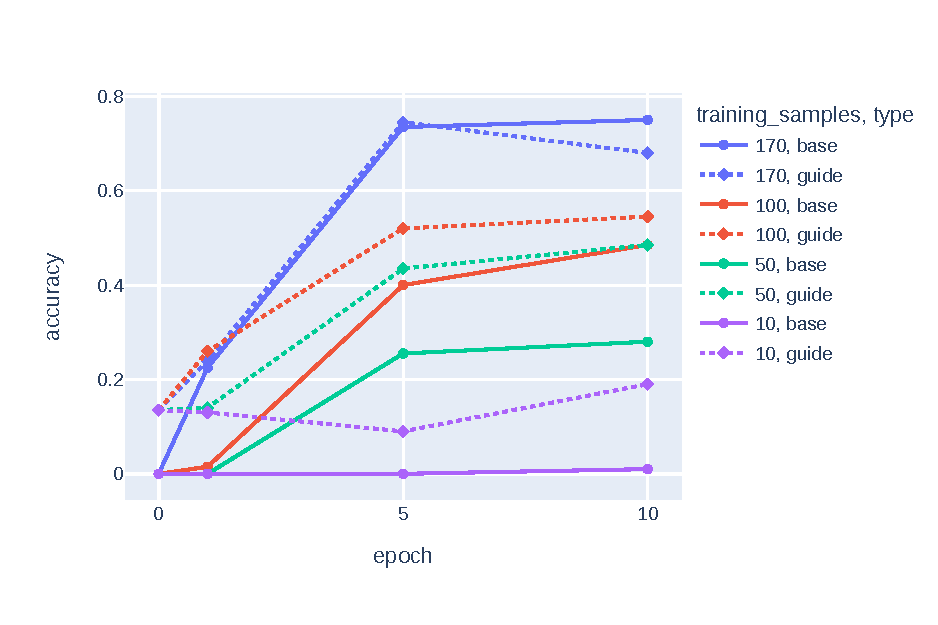
\includegraphics[width=0.45\linewidth]{../plots/accuracy_vs_epoch.pdf}
%        \caption{The accuracy of the Mistral-7B models at different points during the fine-tuning.
%        \emph{Base} refers to the standard ReCOGS dataset after renumbering and \emph{guide}
%        refers to the CoT-enhanced dataset $D^\prime$.
%        }
        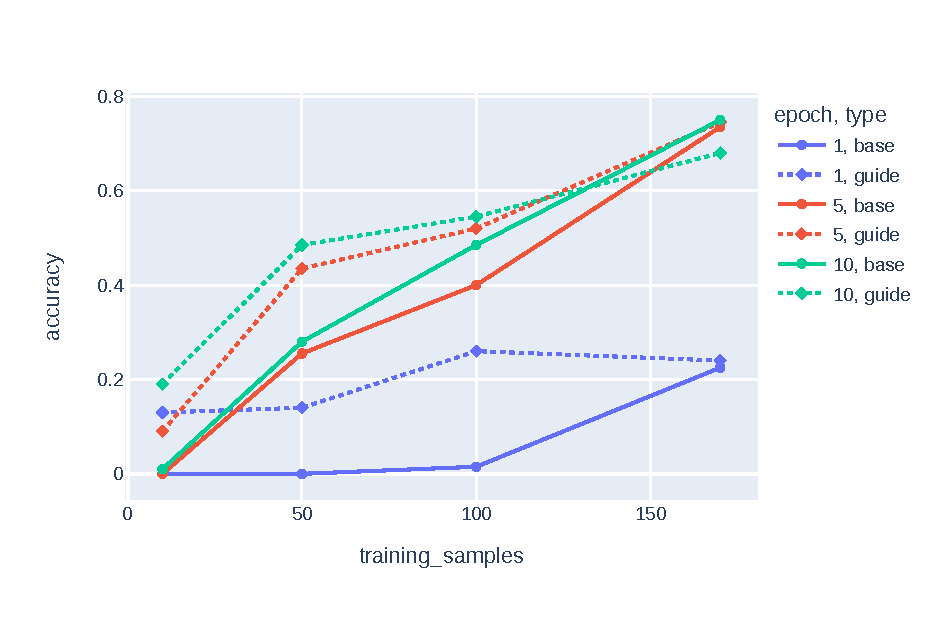
\includegraphics[width=0.45\linewidth]{../plots/accuracy_vs_data.pdf}
        \caption{
            \textbf{Left:} the accuracy of the Mistral-7B models at different points during the fine-tuning.
            \textbf{Right:} the accuracy of the Mistral-7B models with respect to the size of the dataset used for fine-tuning.\\
            In both plots \emph{base} refers to the standard ReCOGS dataset after renumbering and \emph{guide}
            refers to the CoT-enhanced dataset $D^\prime$. The latter case is shown by the dashed lines.
        }
        \label{fig:acc_vs_data_and_epoch}
    \end{figure*}


    \section{Analysis}

    Discussion of what the results mean, what they don’t mean, where they can be improved, etc. These sections vary a lot depending on the nature of the paper. (For papers reporting on experiments with multiple datasets, it can be good to repeats Methods/Results/Analysis in separate (sub)sections for each dataset.)

    \begin{figure*}
        \centering
        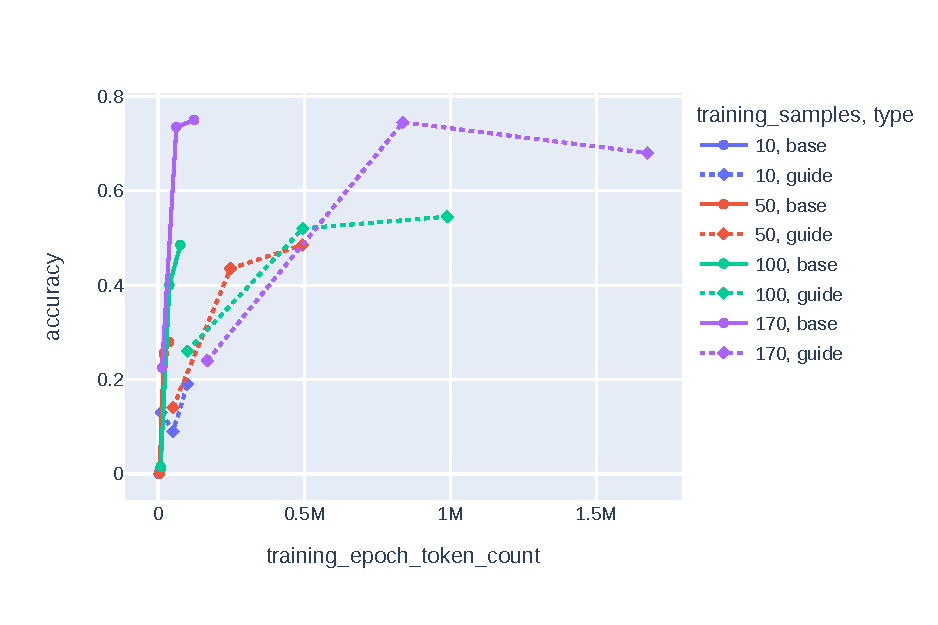
\includegraphics[width=0.45\linewidth]{../plots/accuracy_vs_epochtoken.pdf}
%        \caption{The accuracy of the Mistral-7B models at different points during the fine-tuning.
%        \emph{Base} refers to the standard ReCOGS dataset after renumbering and \emph{guide}
%        refers to the CoT-enhanced dataset $D^\prime$.
%        }
        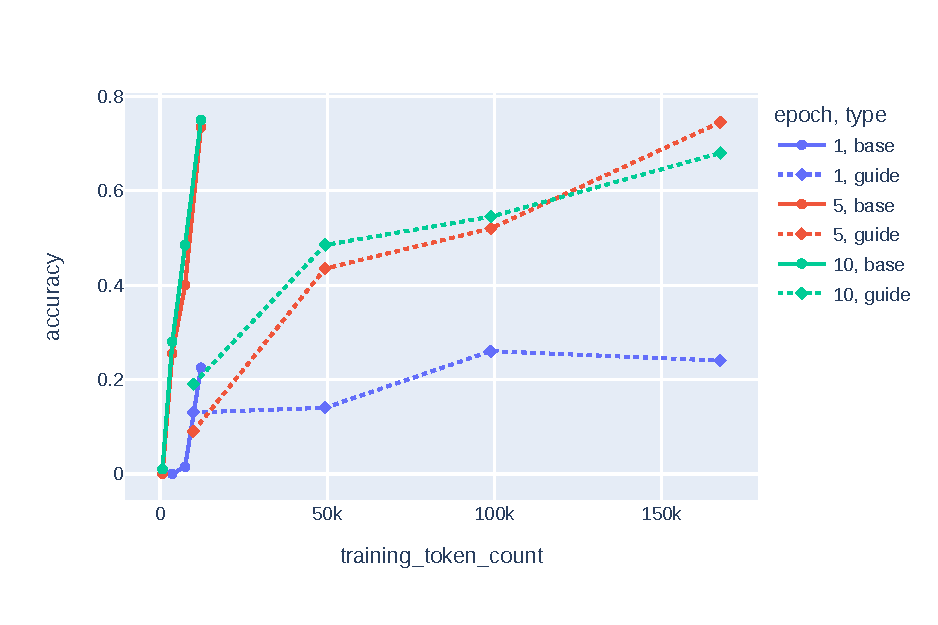
\includegraphics[width=0.45\linewidth]{../plots/accuracy_vs_trainingtoken.pdf}
        \caption{
            \textbf{Left:} the accuracy of the Mistral-7B models at different points during the fine-tuning.
            \textbf{Right:} the accuracy of the Mistral-7B models with respect to the size of the dataset used for fine-tuning.\\
            In both plots \emph{base} refers to the standard ReCOGS dataset after renumbering and \emph{guide}
            refers to the CoT-enhanced dataset $D^\prime$. The latter case is shown by the dashed lines.
        }
        \label{fig:acc_vs_token}
    \end{figure*}

    \section{Conclusion}

    Quickly summarize what the paper did, and then chart out possible future directions that anyone might pursue.

    \begin{itemize}
        \item Focus on GPT-4. What about self generated CoT?
        \item Low statistics
        \item Investigation for bigger training and testing data
        \item Investigate on another dataset
    \end{itemize}

    \section*{Known Project Limitations}

    For this section, imagine that your reader is a well-intentioned NLP practitioner who is seeking to make use of your data, models, or findings as part of a separate scholarly project, deployed system, or some other kind of real-world intervention. What should such a person know about your work? Especially important here are limitations and biases that might affect this person, their findings, their experiment participants, or the users of their product or service. The idea is that what you say here will be taken into consideration but this well-intentioned user, leading to better outcomes for everyone.


    \section*{Authorship Statement}

    Explain how the individual authors contributed to the
    project. You are free to include whatever information you deem important to convey. For ideas and a model see \url{http://blog.pnas.org/iforc.pdf} (p.~12).
    This statement is required even for singly-authored papers, because we want to know whether your project is a collaboration with people outside of the class. Our rationale for this section is that we think this is an important aspect of scholarship in general. Only in extreme cases, and after discussion with the team, would we consider giving separate grades to team members based on this statement.

% Entries for the entire Anthology, followed by custom entries
    \bibliography{anthology,custom,julian}

    \appendix


    \section{Prompts used throughout the project}\label{sec:appendix}
    Throughout this project, specific prompts are used to achieve intermediary results or for training and inference.
    These are reported here for the sake of reproducibility and are shown in figures \ref{fig:guide_prompt},
    \ref{fig:gpt4_recogs_guide}, \ref{fig:prompt_generate_cot_solution}, \ref{fig:gpt4_cot_solution_example} and \ref{fig:prompt_using_guide}.

    \begin{figure*}
        \small
        \texttt{You must come up with a general step by step guide, how to create the logical form from a given sentence.\\
        The guide should also explain the syntax and symbols that the specific logical form requires.\\
        The guide must be compact and use only as many words as are needed to cover all necessary rules.\\
        It must not contain any markdown formatting.\\
        The last step of the guide should only return the full correct logical form.\\
        \\
        Using one of the example pairs, give a demonstration how you use the guide to convert a sentence into its correct logical form.\\
        \\
        -----\\
        Examples:\\
        {\color{red}\{Twenty example pairs are inserted here\}}
        }
        \caption{The prompt sent to GPT-4 to generate a step-by-step guide for solutions of the ReCOGS dataset.}
        \label{fig:guide_prompt}
    \end{figure*}

    \begin{figure*}
        \small
        \begin{verbatim}
Syntax and symbols:
- "*" indicates nonspecific or generalized nouns.
- Numerals (1, 2, 3, ...) are used to uniquely identify nouns and verbs.
- Parentheses are used to group the arguments of functions and relations.
- Semicolons are used to separate independent statements or clauses.

Guide:
1. Identify nouns: Assign each noun a unique numeral (start with 1,
increment for each new noun). If a noun is indefinite or nonspecific,
prefix it with *.

2. Identify the main verb: Assign the next numeral in sequence to the main verb.

3. Determine verb dependencies: For each action (verb), identify its agent (doer),
theme (receiver), or recipient if applicable.
    - Use "agent" for the doer of the action.
    - Use "theme" for the direct object or the focus of the action.
    - Use "recipient" for the indirect object or beneficiary of the action.
    - Use "nmod." for prepositional relations, specifying the relation (e.g.,
        "nmod.in", "nmod.on").

4. Special cases: - For sentences with embedded clauses or secondary actions,
    repeat step 3 for the secondary action within its scope.
    - For sentences indicating possession, use the relation "possessor" and
        "possession".

5. Represent the logical form: - Use semicolon (;) to separate statements.
    - Use parentheses for function arguments, starting with the function
        name (e.g., the verb or relation), followed by the numerical
        identifiers of the relevant nouns.
    - Use "AND" to join multiple conditions or relations related to the same verb.

---
Demonstration with example:

Sentence: "Noah sold a donut to a bear."

Step 1: Identify nouns - Noah ( 1 ); donut ( 2 ); bear ( 3 )
Step 2: Identify the main verb - sold ( 4 )
Step 3: Determine verb dependencies
    - Noah is the agent who performs the action of selling, so he's the "agent".
    - The donut is the item being sold, so it's the "theme".
    - The bear is the recipient of the donut, so it's the "recipient".
Step 4: Special cases: - Not relevant
Step 5: Represent the logical form Noah ( 1 ); donut ( 2 ); bear ( 3 );
    sell ( 4 ) AND agent ( 4 , 1) AND theme ( 4 , 2) AND recipient ( 4 , 3 )
        \end{verbatim}
        \caption{The step-by-step guide generated by GPT-4 for the ReCOGS dataset.}
        \label{fig:gpt4_recogs_guide}
    \end{figure*}

    \begin{figure*}
        \small
        \texttt{
            You are given a sentence and a specific logical form that represents the semantics of the sentence.
            Your task is to follow a step by step guide and generate answers for each of the steps,
            while using as few words as possible.
            The answer to each step should lead to the given logical form, which you return fully in the last step.
            For support, you are also given a demonstration of how to use the step-by-step guide.\\
            -----\\
            Step by step guide and demonstration:\\
            {\color{red}\{The step-by-step guide generated by GPT-4 is inserted here (see fig. \ref{fig:gpt4_recogs_guide})\}.}\\
            -----\\
            Sentence:\\
            {\color{red}\{The sentence for which a step-by-step solution is generated.\}}\\
            Logical Form:\\
            {\color{red}\{The ground truth logical form of the sentence, for which a step-by-step solution is generated.\}}
        }
        \caption{The prompt used to generate a step-by-step solution for a sentence, based on the general guide.}
        \label{fig:prompt_generate_cot_solution}
    \end{figure*}

    \begin{figure*}
        \small
        \begin{verbatim}
Step 1: Identify nouns - cat ( 1 ); *strawberry ( 2 ); pedestal ( 3 ); boy ( 4 )
Step 2: Identify the main verb - lended ( 24 )
Step 3: Determine verb dependencies
    - The cat is the agent of lending, so it's the "agent".
    - The strawberry is the item being lent, so it's the "theme".
    - The boy is the recipient of the strawberry, so it's the "recipient".
    - The strawberry is on the pedestal, which is a prepositional relation.
Step 4: Special cases - The relation between the strawberry and the pedestal
    is specified with "nmod.on".
Step 5: Represent the logical form cat ( 1 ); *strawberry ( 2 ); pedestal ( 3 );
    boy ( 4 ); nmod.on ( 2 , 3 ) AND lend ( 24 ) AND agent ( 24 , 1 ) AND
    theme ( 24 , 2 ) AND recipient ( 24 , 4 )
        \end{verbatim}
        \caption{The step-by-step solution generated by GPT-4 for the sentence
        "A cat lended the strawberry on a pedestal to a boy."}
        \label{fig:gpt4_cot_solution_example}
    \end{figure*}

    \begin{figure*}
        \small
        \texttt{
            You are given a sentence and must convert it to a specific logical form that
            represents the semantics of the sentence. To do this you must follow a step
            by step guide that you are provided with below. You must follow the steps and
            generate answers for each of the steps, while using as few words as possible.
            The answer to each step should lead to the logical form, which you return in
            the last step. For support, you are also given an example of how to use the
            step by step guide to convert a given sentence to its logical form.\\
            \\
            -----\\
            Step by step guide and demonstration:\\
            {\color{red}\{The step-by-step guide generated by GPT-4 is inserted here (see fig. \ref{fig:gpt4_recogs_guide})\}}\\
            \\
            -----\\
            Sentence to convert:\\
            {\color{red}\{The sentence to convert is inserted here.\}}
        }
        \caption{The prompt used for inference, for the case with CoT-style solution.}
        \label{fig:prompt_using_guide}
    \end{figure*}

\end{document}
